\begin{definition}\label{def:rrgp}
Let $\pi=\pi_1^{(x_1,y_1)}\pi_2^{(x_2,y_2)}\dotsm\pi_n^{(x_n,y_n)} \in \mathcal{G}_n$ and define its \emph{column reverse} for $[a,b]$ where $a,b\in\N$ and $a\leq b$ as the mapping $\textsf{rev}_{[a,b]}$ where $\textsf{rev}_{[a,b]}(\pi)$ is $\pi$ where its longest subsequence whose columns all belong to interval
\[
\pi_{i}^{(x_i,y_i)}\pi_{i+1}^{(x_{i+1},y_{i+1})}\dotsm\pi_{i+k}^{(x_{i+k},y_{i+k})}
\]
has been replaced by 
\[
    \pi_{i+k}^{(a+b-x_{i+k},y_{i+k})}\dotsm\pi_{i+1}^{(a+b-x_{i+1},y_{i+1})}\pi_{i}^{(a+b-x_i,y_i)}.
\]
\end{definition}

The column reverse can be extended to subsequences of gridded permutations and tilings such that it is applied to all of its obstructions and requirements. Suppose $\pi = 5^{(0,1)}2^{(0,0)}4^{(1,1)}1^{(1,0)}6^{(2,2)}3^{(3,1)}$, then 
\[
\textsf{rev}_{[1,2]}(\pi) = 5^{(0,1)}2^{(0,0)}6^{(1,2)}1^{(2,0)}4^{(2,1)}3^{(3,1)},
\]
as shown in \FigureRef{fig:gp_col_rev}. An example for tilings can be seen in \FigureRef{fig:t_col_rev}.

\begin{figure}[ht!]
    \centering
    {
\newcommand{\picw}{1}
\newcommand{\pich}{1}
\begin{tikzpicture}
    \fill[gray!20] (\picw,0) rectangle (3*\picw,3*\pich);
    \draw (1 * \picw, 0) -- (1 * \picw, \pich * 3);
    \draw (2 * \picw, 0) -- (2 * \picw, \pich * 3);
    \draw (3 * \picw, 0) -- (3 * \picw, \pich * 3);
    \draw (0, 1 * \pich) -- (4 * \picw, 1 * \pich);
    \draw (0, 2 * \pich) -- (4 * \picw, 2 * \pich);
    \draw[rounded corners=2ex] (0,0) rectangle (4*\picw,3*\pich);
    \draw (0.25*\picw,3.5*0.5*\pich) -- (0.75*\picw,1*0.5*\pich) -- (1.25*\picw,3*0.5*\pich) -- (1.75*\picw,0.5*0.5*\pich) -- (2.5*\picw,5*0.5*\pich) -- (3.5*\picw,2.5*0.5*\pich);
    \fill (0.25*\picw,3.5*0.5*\pich) circle (0.075) node[below] {$5$};
    \fill (0.75*\picw,1*0.5*\pich) circle (0.075) node[below] {$2$};
    \fill (1.25*\picw,3*0.5*\pich) circle (0.075) node[above] {$4$};
    \fill (1.75*\picw,0.5*0.5*\pich) circle (0.075) node[left] {$1$};
    \fill (2.5*\picw,5*0.5*\pich) circle (0.075) node[above] {$6$};
    \fill (3.5*\picw,2.5*0.5*\pich) circle (0.075) node[above] {$3$};
\end{tikzpicture}
\begin{tikzpicture}
    \draw[white] (0,0) rectangle (2,3*\pich);
    \draw[thick, ->] (0.25,1.5*\pich) -- (1.75,1.5*\pich) node[above,pos=.5] {$\textsf{rev}_{[1,2]}$};
\end{tikzpicture}
\begin{tikzpicture}
    \fill[gray!20] (\picw,0) rectangle (3*\picw,3*\pich);
    \draw (1 * \picw, 0) -- (1 * \picw, \pich * 3);
    \draw (2 * \picw, 0) -- (2 * \picw, \pich * 3);
    \draw (3 * \picw, 0) -- (3 * \picw, \pich * 3);
    \draw (0, 1 * \pich) -- (4 * \picw, 1 * \pich);
    \draw (0, 2 * \pich) -- (4 * \picw, 2 * \pich);
    \draw[rounded corners=2ex] (0,0) rectangle (4*\picw,3*\pich);
    \draw (0.25*\picw,3.5*0.5*\pich) -- (0.75*\picw,1*0.5*\pich) -- (1.5*\picw,5*0.5*\pich) -- (2.25*\picw,0.5*0.5*\pich) -- (2.75*\picw,3*0.5*\pich) -- (3.5*\picw,2.5*0.5*\pich);
    \fill (0.25*\picw,3.5*0.5*\pich) circle (0.075) node[below] {$5$};
    \fill (0.75*\picw,1*0.5*\pich) circle (0.075) node[below] {$2$};
    \fill (1.5*\picw,5*0.5*\pich) circle (0.075) node[above] {$6$};
    \fill (2.25*\picw,0.5*0.5*\pich) circle (0.075) node[right] {$1$};
    \fill (2.75*\picw,3*0.5*\pich) circle (0.075) node[above] {$4$};
    \fill (3.5*\picw,2.5*0.5*\pich) circle (0.075) node[above] {$3$};
\end{tikzpicture}
}
    \caption{The column reverse of a gridded permutation.}
    \label{fig:gp_col_rev}
\end{figure}

\begin{figure}[ht!]
    \centering
    
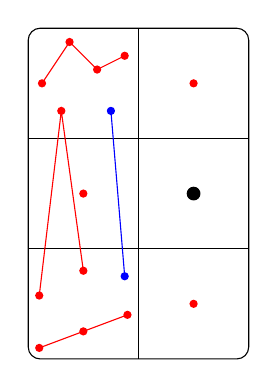
\begin{tikzpicture}[scale=0.7, every node/.style={scale=0.7}]
	\fill (3,3) circle (0.125);
	\fill[red] (1,3) circle (0.075);
	\fill[red] (3,5) circle (0.075);
	\fill[red] (3,1) circle (0.075);
    \draw[rounded corners=1ex] (0,0) rectangle (4,6);
    \draw (0,2) -- (4,2);
    \draw (0,4) -- (4,4);
    \draw (2,0) -- (2,6);
	\coordinate (a1) at (0.2,0.2);
	\coordinate (a2) at (1,0.5);
	\coordinate (a3) at (1.8,0.8);
	\coordinate (b1) at (0.2,1.15);
	\coordinate (b2) at (0.6,4.5);
	\coordinate (b3) at (1,1.6);
	\coordinate (c1) at (0.25,5);
	\coordinate (c2) at (0.75,5.75);
	\coordinate (c3) at (1.25,5.25);
	\coordinate (c4) at (1.75,5.5);
	\coordinate (d1) at (1.5,4.5);
	\coordinate (d2) at (1.75,1.5);
	\fill[red] (a1) circle (0.075);
	\fill[red] (a2) circle (0.075);
	\fill[red] (a3) circle (0.075);
	\fill[red] (b1) circle (0.075);
	\fill[red] (b2) circle (0.075);
	\fill[red] (b3) circle (0.075);
	\fill[red] (c1) circle (0.075);
	\fill[red] (c2) circle (0.075);
	\fill[red] (c3) circle (0.075);
	\fill[red] (c4) circle (0.075);
	\fill[blue] (d1) circle (0.075);
	\fill[blue] (d2) circle (0.075);
	\draw[red] (a1) -- (a2) -- (a3);
	\draw[red] (b1) -- (b2) -- (b3);
	\draw[red] (c1) -- (c2) -- (c3) -- (c4);
	\draw[blue] (d1) -- (d2);
\end{tikzpicture}
\begin{tikzpicture}[scale=0.7]
	\draw[white] (0,0) rectangle (2,6);
	\draw[thick, ->] (-.5,3) -- (2.5,3) node[above,pos=.5] {$\textsf{rev}_{[0,0]}$};
\end{tikzpicture}
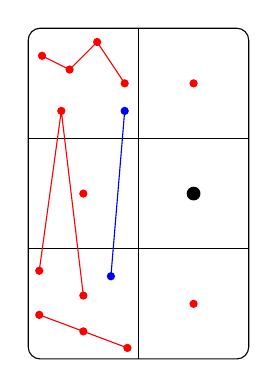
\begin{tikzpicture}[scale=0.7, every node/.style={scale=0.7}]
	\fill (3,3) circle (0.125);
	\fill[red] (1,3) circle (0.075);
	\fill[red] (3,5) circle (0.075);
	\fill[red] (3,1) circle (0.075);
    \draw[rounded corners=1ex] (0,0) rectangle (4,6);
    \draw (0,2) -- (4,2);
    \draw (0,4) -- (4,4);
    \draw (2,0) -- (2,6);
	\coordinate (a1) at (1.8,0.2);
	\coordinate (a2) at (1,0.5);
	\coordinate (a3) at (0.2,0.8);
	\coordinate (b1) at (1,1.15);
	\coordinate (b2) at (0.6,4.5);
	\coordinate (b3) at (0.2,1.6);
	\coordinate (c1) at (1.75,5);
	\coordinate (c2) at (1.25,5.75);
	\coordinate (c3) at (0.75,5.25);
	\coordinate (c4) at (0.25,5.5);
	\coordinate (d1) at (1.75,4.5);
	\coordinate (d2) at (1.5,1.5);
	\fill[red] (a1) circle (0.075);
	\fill[red] (a2) circle (0.075);
	\fill[red] (a3) circle (0.075);
	\fill[red] (b1) circle (0.075);
	\fill[red] (b2) circle (0.075);
	\fill[red] (b3) circle (0.075);
	\fill[red] (c1) circle (0.075);
	\fill[red] (c2) circle (0.075);
	\fill[red] (c3) circle (0.075);
	\fill[red] (c4) circle (0.075);
	\fill[blue] (d1) circle (0.075);
	\fill[blue] (d2) circle (0.075);
	\draw[red] (a1) -- (a2) -- (a3);
	\draw[red] (b1) -- (b2) -- (b3);
	\draw[red] (c1) -- (c2) -- (c3) -- (c4);
	\draw[blue] (d1) -- (d2);
\end{tikzpicture}
    \caption{The column reverse of a tiling.}
    \label{fig:t_col_rev}
\end{figure}

\begin{lemma}\label{lem:crevcontain}
Let $\pi, \sigma \in \mathcal{G}$ such that $\contains{\pi}{\sigma}$, then $\contains{\textsf{rev}_{[a,b]}(\pi)}{\textsf{rev}_{[a,b]}(\sigma)}$.
\end{lemma}
\begin{proof}
If $\pi$ has no elements within the columns then neither does $\sigma$ and both are mapped to themselves. If $\sigma$ has no elements within the columns then the mapping has no effect on the pattern which remains in $\textsf{rev}_{[a,b]}(\pi)$. 

Let $\set{i,i+1,\dotsc,i+k}$ be the indices of elements of $\pi$ with columns in $[a,b]$. Let $\sigma = \st{\sseq{A_1\cup L \cup A_2}{\pi}}$ where $L \subseteq \set{i,i+1,\dotsc,i+k}$ and $A_1$ and $A_2$ are the indices in $\pi$ on either side of the columns corresponding to the occurrence of $\sigma$, then
\begin{align*}
    \textsf{rev}_{[a,b]}(\sigma) &= \textsf{rev}_{[a,b]}\left(\st{\sseq{A_1\cup L \cup A_2}{\pi}}\right)\\ 
    &= \st{\textsf{rev}_{[a,b]}\left(\sseq{A_1\cup L \cup A_2}{\pi}\right)}\\
    &= \st{\textsf{rev}_{[a,b]}\left(\sseq{A_1}{\pi}\sseq{L}{\pi}\sseq{A_2}{\pi}\right)}\\
    &= \st{\sseq{A_1}{\pi}\textsf{rev}_{[a,b]}\left(\sseq{L}{\pi}\right)\sseq{A_2}{\pi}} \\
    &= \st{\sseq{A_1}{\textsf{rev}_{[a,b]}(\pi)}\textsf{rev}_{[a,b]}\left(\sseq{L}{\pi}\right)\sseq{A_2}{\textsf{rev}_{[a,b]}(\pi)}} \\
    &= \st{\sseq{A_1}{\textsf{rev}_{[a,b]}(\pi)}\sseq{\cset{2i+k-\ell}{\ell \in L}}{\textsf{rev}_{[a,b]}(\pi)}\sseq{A_2}{\textsf{rev}_{[a,b]}(\pi)}}\\
    &= \st{\sseq{A_1 \cup \cset{2i+k-\ell}{\ell \in L} \cup A_2}{\textsf{rev}_{[a,b]}(\pi)}}
\end{align*}
which shows that $\textsf{rev}_{[a,b]}(\sigma)$ is the standardization of a subsequence of $\textsf{rev}_{[a,b]}(\pi)$.
\end{proof}

\begin{lemma}\label{lem:crevgrid}
Let $\mathcal{T}$ be a tiling and $\pi \in \textsf{Grid}(\mathcal{T})$, then $\textsf{rev}_{[a,b]}(\pi)\in\textsf{Grid}(\textsf{rev}_{[a,b]}(\mathcal{T}))$.
\end{lemma}
\begin{proof}
By Lemma \ref{lem:crevcontain} all occurrences of requirements are preserved so the only way that $\textsf{rev}_{[a,b]}(\pi)$ is not in $\textsf{Grid}(\textsf{rev}_{[a,b]}(\mathcal{T}))$ is if there exists an obstruction $o$ that is avoided by $\pi$ while $\textsf{rev}_{[a,b]}(\pi)$ contains $\textsf{rev}_{[a,b]}(o)$. Suppose that there is such an obstruction, then $\textsf{rev}_{[a,b]}(\textsf{rev}_{[a,b]}(\pi)) = \pi$ must contain $\textsf{rev}_{[a,b]}(\textsf{rev}_{[a,b]}(o)) = o$ which contradicts $\pi$ avoiding $o$.
\end{proof}

\begin{proposition}\label{prop:rrtil}
Let $\mathcal{T}$ be a tiling, then $|\textsf{Grid}_n(\mathcal{T})| = |\textsf{Grid}_n(\textsf{rev}_{[a,b]}(\mathcal{T}))|$ for all $n\in\N$.
\end{proposition}
\begin{proof}
With $\textsf{rev}_{[a,b]}$ being its own inverse it is a bijection between $\textsf{Grid}_n(\mathcal{T})$ and
\[
\cset{\textsf{rev}_{[a,b]}(\pi)}{\pi \in \textsf{Grid}_n(\mathcal{T})}
\]
with the latter being a subset of $\textsf{Grid}_n(\textsf{rev}_{[a,b]}(\mathcal{T}))$ by Lemma \ref{lem:crevgrid} and therefore we have $|\textsf{Grid}_n(\mathcal{T})| \leq |\textsf{Grid}_n(\textsf{rev}_{[a,b]}(\mathcal{T}))|$. By the same argument there is a bijection between $\textsf{Grid}_n(\textsf{rev}_{[a,b]}(\mathcal{T}))$ and
\[
    \cset{\textsf{rev}_{[a,b]}(\pi)}{\pi \in \textsf{Grid}_n(\textsf{rev}_{[a,b]}(\mathcal{T}))}
\]
with the latter being a subset of $\textsf{Grid}_n(\textsf{rev}_{[a,b]}(\textsf{rev}_{[a,b]}(\mathcal{T})))=\textsf{Grid}_n(\mathcal{T})$ and therefore $|\textsf{Grid}_n(\mathcal{T})| \geq |\textsf{Grid}_n(\textsf{rev}_{[a,b]}(\mathcal{T}))|$ and thus $|\textsf{Grid}_n(\mathcal{T})| = |\textsf{Grid}_n(\textsf{rev}_{[a,b]}(\mathcal{T}))|$
\end{proof}